\documentclass[12pt,a4paper]{article}
\usepackage[a4paper,left=1.0in,right=1.0in,top=1.0in,bottom=1.0in]{geometry}
\usepackage[utf8]{inputenc}
\usepackage[T1]{fontenc}
\usepackage{amsmath}
\usepackage{amsfonts}
\usepackage{amssymb}
\usepackage{graphicx}
\usepackage{cite}
\usepackage{hyperref}
\usepackage{mdframed}
\usepackage{multicol}
\usepackage{pdfpages}


\graphicspath{{./images/}}

\hypersetup{
	colorlinks=true,
	linkcolor=blue,
	filecolor=magenta,      
	urlcolor=cyan,
}

\usepackage{listings}
\usepackage{xcolor}
\definecolor{codegreen}{rgb}{0,0.6,0}
\definecolor{codegray}{rgb}{0.5,0.5,0.5}
\definecolor{codepurple}{rgb}{0.58,0,0.82}
\definecolor{backcolour}{rgb}{0.95,0.95,0.92}

\lstdefinestyle{mystyle}{
	backgroundcolor=\color{backcolour},   
	commentstyle=\color{codegreen},
	keywordstyle=\color{magenta},
	numberstyle=\tiny\color{codegray},
	stringstyle=\color{codepurple},
	basicstyle=\ttfamily\small,
	breakatwhitespace=false,         
	breaklines=true,                 
	captionpos=b,                    
	keepspaces=true,                 
	numbers=left,                    
	numbersep=5pt,                  
	showspaces=false,                
	showstringspaces=false,
	showtabs=false,                  
	tabsize=2
}
\lstset{style=mystyle}


\begin{document}
\section{Pourtsidou et al. 2014}
\subsection{Cosmology and parameters}
\subsubsection{Cosmology}
Parameters taken from Table 2 (68\% limits) of Planck 2013. 
\begin{align*}
	h &= 0.673\\
	\Omega_{m_0} &= 0.315\\
	\Omega_{b} &= 0.02205/h^2\\
	\Omega_{c} &= 0.1199/h^2\\
	\Omega_{l} &= 0.685\\
	As &= 2.196\times 10^{-9}\\
	n_s &= 0.9603\\
	Y_{He} &= 0.24770\\
	\sigma_8 &= 0.829\\
\end{align*}
%\begin{lstlisting}[language=python]
%from scipy.special import gamma
%h = 0.673
%omegab = 0.02205 / h**2
%omegac = 0.1199 / h**2
%omegam = 0.315
%omegal = 0.685
%ns = 0.9603
%As = 2.196 * 10**(-9)
%sigma_8 = 0.829
%YHe = 0.24770 #-- Y_p in the paper
%
%
%#-- parameters stated below equation in Pourtsidou et al. 2014
%
%T_sys = 50 #-- kelvin 
%t_obs = 2 * 365 * 24 * 3600 #-- seconds
%bandwidth = 40 #-- MHz
%l_max = 19900
%f_cover = 0.06
%delta_l = 36
%f_sky = 0.2
%
%## To calculate Tz(z)
%#-- Refer to eq. 1 and eq. 17-19 of P_2014
%alpha = -1.3
%phi_star = 0.0204 * h**3 #-- Mpc^(-3)
%m_star = 3.47 * 10**9 / h**2 #-- solar mass
%rho_c = 2.7755 * h**2 * 10**11
%
%### mean galaxy number density 
%#-- defined near equation 9 of P_2014
%eta_bar = phi_star * gamma(alpha + 1)
%
%### mean and relative HI galaxy mass density 
%#-- equation 18 in P_2014
%#-- mean
%rhoHI = phi_star * m_star * gamma(alpha + 2)
%#-- relative
%omegaH1 = rhoHI / rho_c
%
%### mass moments
%#-- defined near eq. 9 of P_2014 
%#-- Required in equation 14 of P_2014
%mass_moment_1 = phi_star * m_star * gamma(alpha + 2) / eta_bar
%mass_moment_2 = phi_star * m_star**2 * gamma(alpha + 3) / eta_bar
%mass_moment_3 = phi_star * m_star**3 * gamma(alpha + 4) / eta_bar
%mass_moment_4 = phi_star * m_star**4 * gamma(alpha + 5) / eta_bar
%
%\end{lstlisting}

\subsubsection{Experimental parameters}
Parameters of SKA-like experiment used in P2014. 
\begin{align*}
T_{sys} &= 50\;K\\
t_{obs} &= 2\; years\\
Bandwidth &= 40\;MHz \\
l_{max} &= 19900\\
f_{cover} &= 0.06\\
\Delta_L &= 36\\
f_{sky} &= 0.2\\
%\Omega_{HI} &= 0.7
\end{align*}

\paragraph{Other parameters}
To calculate $ \bar{T}(z) $. Refer to Eq. 1 and Eq. 17-19 of P2014.
\begin{align*}
\alpha &= -1.3\\
\phi^\star &= 0.0204 h^3 \; Mpc^{-3} \\
M^\star &= \frac{3.47\times10^9}{h^2}M_\odot \\
\rho_c &= 2.7755 \times 10^{11} h^2 M_\odot Mpc^{-3}\\
\rho_{HI} &= \phi^\star M^\star \Gamma(\alpha + 2)  \\
\Omega_{HI}(z) &= \rho_{HI}/\rho_c = 0.0004919
\end{align*}
The parameter $ \Omega_{HI} $ is a function of $ z $ but I can't see how. Are $ M^\star $ and $ \phi^\star $ dependent on $ z $? $ \rho_c $ is the present day critical density so this is not bringing in the $ z $ dependence. If we look at the units of $ \Omega_{HI} $, we get.
\begin{align}
\Omega_{HI}(z) &= \frac{\rho_{HI}}{\rho_c} \\
&\propto \frac{\phi^\star M^\star \Gamma(\alpha + 2)}{\rho_c}\\
&\propto \frac{h^3 Mpc^{-3} \times h^{-2}M_\odot}{h^2 M_\odot Mpc^{-3}}\\
&\propto \frac{1}{h},
\end{align}
Do we expect this $ h $ dependence of $ \Omega_{HI} $?

\subsection{$ T_{HI} $}
The mean $ HI $ intensity temperature at redshift z (Eq. 1 of P2014) is written as
\begin{align}
\bar{T}(z) = 180 \Omega_{HI}(z) h \frac{(1 + z)^2}{E(z)}\delta \; \mathrm{mK}
\end{align}
where $ h = H_0 / (100 kms^{-1}Mpc^{-1})$, $ \Omega_{HI} $ is the average $ HI $ density at redshift z realtive to the present day critical density. Fig. \ref{fig:tz-vs-z} shows the variation of $ \bar{T}(z) $ with $ z $.
\begin{figure}
	\centering
	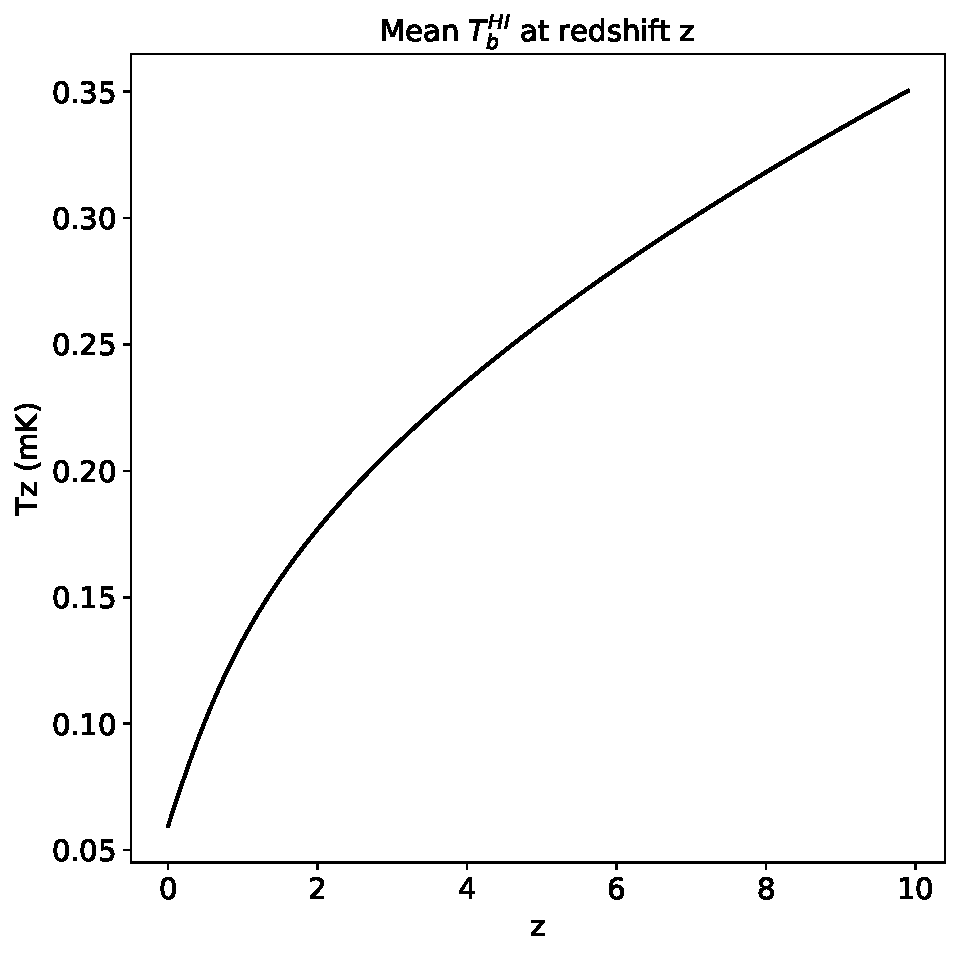
\includegraphics[width=0.7\textwidth]{variation-of-tz-with-z}
	\caption{Variation of $ HI $} brightness temperature with redshift. 
	\label{fig:tz-vs-z}
\end{figure}
Here and in Eq. 20 of P2014 I have taken
\begin{align}
E(z) &= \frac{H(z)}{H_0}\\
&= \sqrt{\Omega_{m_0} (1 + z)^3 + \Omega_{l}}.
\end{align}

\subsection{Matter power spectrum}
I have used the following code to obtain the matter power spectrum using Python CAMB.
\begin{lstlisting}[language=python]
pars = model.CAMBparams(NonLinear = 0, WantTransfer = True, H0 = 100 * h, omch2 = omegach2, ombh2 = omegabh2, YHe = YHe)
pars.DarkEnergy.set_params(w = -1)
pars.set_for_lmax(lmax = l_ul)
pars.InitPower.set_params(ns = ns, As = As)
#results = camb.get_background(pars)
results = camb.get_results(pars)
k = np.linspace(10**(-5), k_max(l_ul, z_s) ,1000)
PK = get_matter_power_interpolator(pars, nonlinear=False, kmax = np.max(k), k_hunit = False, hubble_units = False)
\end{lstlisting}

Some of the important parameters are:
\begin{itemize}
	\item \verb|NonLinear = 0|: Out of the four options available in CAMB for choosing the type of power spectrum, \verb|0| gives linear power spectrum with $ \sigma_8 \sim 0.8$ (so the normalization is correct), \verb|1| gives ``Non-linear Matter Power (HALOFIT)" and the other two have CMB in their name so we don't care. The \verb|nonlinear = False| also specifies that we wanr to generate a linear power spectrum. Before the thesis submission we were using \verb|NonLinear = 1| and \verb|nonlinear = True|, and that's why our convergence angular power spectrum was not matching with that of P2014. 
	\item \verb|k_unit = False| and \verb|hubble_units = False|: Read \verb|k| in Mpc units and output the power spectrum in Mpc units. \verb|True| will enable Mpc/h units.
	\item \verb|WantTransfer = True|: I need to find out what this option does, and if I can drop it. I am using this flag since the beginning.
	\item \verb|results = camb.get_background(pars)| and \verb|results = camb.get_results(pars)|: I am not sure what's the difference between the two; both work. I was using \verb|get_background| since the beginning because it is used in \href{https://camb.readthedocs.io/en/latest/CAMBdemo.html}{this CAMB demo}. I switched to \verb|get_results| because it can be used to find $\sigma_8$ by doing \verb|results.get_sigma8()| after we have defined what \verb|results| is as shown in the code.
	\item \verb|l_ul|: It is the upper limit in $ \int d^2l $ integrals in the lensing noise reconsruction expression (Eq. 14 of P2014). It is different from $ l_{max} $ defined in P2014 as the highest multipole visible to the instrument ($ l_{max}  = 19900 $ in P2014). The integrals, I think, should ideally go upto $ l = \infty $, so I usually take \verb|l_ul = 70000| or higher. We need to take such large number because we have 21-cm power spectrum terms in the noise expression. I think that if we take a smaller value for \verb|set_for_lmax| then the power spectrum would not be correct for large \verb|l| values of the integral.
\end{itemize}
Figure \textbf{BlaBla} shows the plot of matter power spectrum $ P_\delta(k) $ as a function of $ k $.


\subsection{Power spectrum of 21-cm line}
Defining the 21-cm power spectrum using Eq. 2 of P2014 as 
\begin{align}
P_{\Delta T_b}(k) = [\bar{T}(z)]^2 (1 + f\mu_k^2)P_\delta(k),
\end{align}
where $ P_\delta(k) $ is the underlying (dark) matter power spectrum, $ f = \frac{d\;ln\; D}{ln\;a}$, $ D $ is the linear growth rate and $ \mu_k$ is the cosine of the angle between wavevector $ \textbf{k} $ and the line of sight $ \hat{z} $, and $ a $ is the scale factor $ (1 + z)^{-1} $.


I have ignored $ (1 + f\mu_k^2) $ in my calculations. The resulting 21-cm power spectrum is shown in Figure \textbf{add figure}.


\subsection{Signam-to-noise ratio}
\subsubsection{Signal}
Prior to the thesis submission I hadn't really figured out how we are choosing our signal. I think I have now understood the concept of signal and noise in the context of lensing reconstruction. It's the following.

\begin{figure}[tbp]
	\centering
	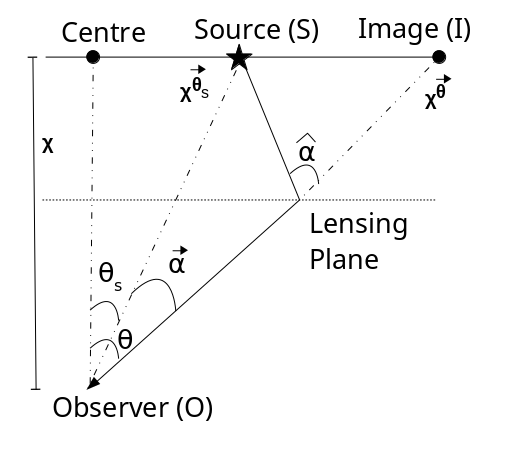
\includegraphics[width = 0.5\textwidth]{lensing_schematic}
	\caption{Schematic of a typical lensing setup. Only one lensing plane is shown for simplicity. Practically, the volume between the observer and the source can be thought of as a stack of many such planes of a certain thickness depending on the bin size we choose.}
	\label{fig:lensing_schematic}
\end{figure}

Figure \ref{fig:lensing_schematic} shows a typical lensing setup. The source is located at a transverse comoving distance \footnote{As per the definition given in Hogg 2006.} $ \chi $ away from the observer. The vector sign in $ \chi^{\vec{\theta}} $ signifies that there are two components of the transverse distance $ \chi^{\vec{\theta}} $ in the source plane -- one in the plane of the paper and the other perpendicular to it. Here, $ \hat{\alpha} $ is called deflection angle and $ \vec{\alpha} $ is called reduced deflection angle. We'll just need $ \vec{\alpha} $ to understand our signal.

Knowledge of $ \vec{\alpha} $ gives the observer the ability to map the images to the source. In other words, the observer reverses the lensing to obtain an unlensed distribution of sources. If we solve the  geodesic equation for the above set up, assuming perturbed FLRW metric, we get

\begin{align}
\vec{\alpha} =  \vec{\bigtriangledown}_{\theta}  \int_{0}^{\chi_s} d\chi^{\prime} \frac{2}{c^2}\Phi(\theta, \chi') \left(\frac{\chi_s - \chi^{\prime}}{\chi'  \chi_s}\right)  = \vec{\bigtriangledown}_{\theta} \psi, \label{eq:deflection_angle}
\end{align}
where $ \chi' $ represents the position of a particular lensing plane relative to the observer, $\Phi$ is the actual gravitational potential due to the mass distribution, and $\psi$ is called lensing potential.

But the problem is that we don't know $ \vec{\alpha} $ for any distribution. CONCERTO is going to record the mass distribution and shape features in its data and we can't find $ \vec{\alpha} $ from that data directly. So we need to relate $ \vec{\alpha} $ to another quantity that can be computed from the data.

Figure \ref{fig:lensing_schematic} gives
\begin{align}
\theta - \theta_s =  \vec{\alpha}
\end{align}
The following Jacobi matrix then gives the map to go from the source to the image. It basically tells us about the transformations by which the image differs from the shape of source.


\begin{align}
\mathcal{A}_{ij}(\chi_S, \theta) &\equiv \frac{\partial\theta_S^i}{\partial\theta^j} \\ 
&= \delta_{ij} - \psi,_{ij} \\
\implies
\mathcal{A} &= \underbrace{(1-\kappa) 
	\begin{pmatrix}
	1 & 0 \\
	0 & 1 \\
	\end{pmatrix}}_{isotropic}
+
\underbrace{
	\begin{pmatrix}
	- \gamma_1 & -\gamma_{2} \\
	-\gamma_{2} & \gamma_1 \\
	\end{pmatrix} 
}_{anisotropic} \label{eq:jacobi}
\end{align}

Here $\gamma_i$ are the components of shear and $ \kappa $ is convergence. Since we are dealing with cosmological weak lensing, we ignore the contribution from shear and take the isotropic term only. I am sure there's a better explanation for this, like convergence and shear are almost the same for weak lensing, but I am not going into that for now.

\paragraph{Question} When we say that we using taking convergence power spectrum 
in our calculations, does it mean that we are ignoring shear in the sense that it's not even there? Or does it mean that we are not considering the effect of shear on the map but it's there, and we are just looking at the effect of convergence?

\begin{figure}[tbp]
	\centering
	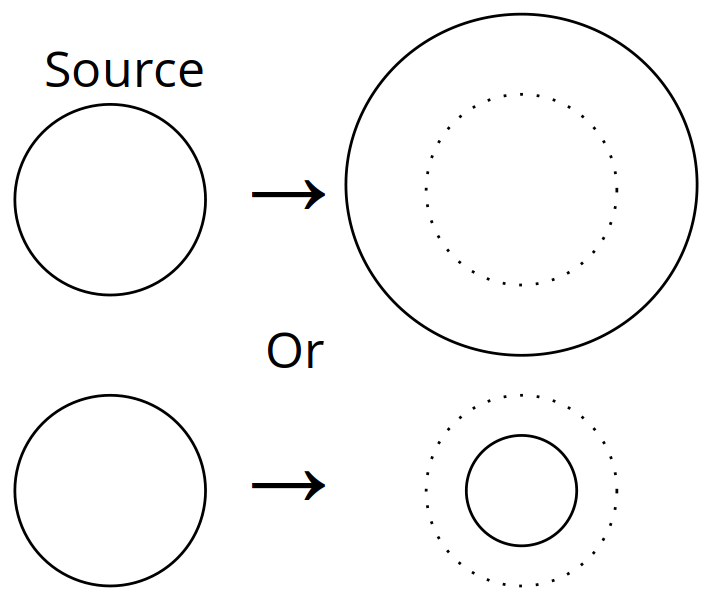
\includegraphics[width=0.5\textwidth]{convergence}
	\caption{Effect of convergence -- magnification for $ \kappa < 1 $ and demagnification for $ \kappa > 1$.}
	\label{fig:convergence}
\end{figure}

Figure \ref{fig:convergence} shows the effect of convergence for positive and negative values of $ \kappa $ in Eq. \eqref{eq:jacobi}. From this figure we see that convergence is a quantity that can be measured from the intensity mapping data (more on this later). Therefore, if we can relate $ \alpha $  with $ \kappa $ then the statistics of $\kappa$ will also be applicable to $ \alpha $.
%Let's assume that we are looking at one slice of the 3D volume that CONCERTO scan. In that sheet, on average, the size of the "structural features" is going to have some distribution

$\kappa$ is defined as 
\begin{align}
\kappa(\theta, \chi) = \frac{1}{2} \vec{\bigtriangledown}_\theta \cdot \vec{\alpha}(\theta, \chi).
\end{align}
Using this realation, we have connected a quantity $\vec{\alpha}$, which couldn't be computed from the data, with a quantity that can be computed via different statistical methods.

The quantity that we have chosen to compute is the power spectrum $ P^\kappa(k) $ of convergence, which is just the two-point correlation function of $\kappa$ in Fourier space. Assuming that $ \vec{l} $ is the Fourier conjugate to position $ \vec{\theta} $, we can write the angular power spectrum of the two quantities as 
\begin{align}
C^{\kappa\kappa}(L) &= \frac{1}{4}L(L+1) C^{\alpha\alpha}(L),\\
\implies C^{\alpha\alpha}(L) &= \frac{4}{L(L+1)} C^{\kappa\kappa}(L) \label{eq:disp_field_pow_spec}
\end{align}
where $ L $ is the observed Fourier mode. 

\paragraph{Error in thesis}Figure \eqref{eq:disp_field_pow_spec} is the reason for why we have $ 4/L(L + 1) $ in equation 20 of P2014. 

Eq. \eqref{eq:disp_field_pow_spec} gives us the statistic we wanted. We can now compute the displacement angle power spectrum from CONCERTO's data indirectly using convergence $\kappa$. So the final expression of our signa (in Pourtsidou's notation) is 
\begin{align}
	C^{\alpha\alpha}(L) \equiv C^{\delta\theta\delta\theta}(L) = \frac{9 H_0^4 \Omega_{m0}^2}{L(L+1)c^4}  \int_0^{\chi_s} d\chi' \left[ \frac{(\chi_s - \chi')}{\chi_s} \frac{1}{a} \right]^2 P_\delta\left( \frac{L}{\chi'}\right).
\end{align}
%What I submitted in the thesis is $ C^{\kappa\kappa} $. That's wrong because I did not make the corresponding changes to the lensing estimator and noise expression, and that messed up the units. The signal (convergence power spectrum) was in dimensionless units and the noise had dimensions of $ energy/c^2 $ (Eq. \eqref{eq:deflection_angle}).

\subsubsection{Noise}
Just like we have found a quantity $ \kappa $ to indirectly measure the deflection angle power spectru, we also need to find the noise in the measurement of $ \vec{\alpha} $. That 





























\end{document}